% !TeX root = ../main.tex
%% =======================================================================
%  CAPITULO 3 — EL CANAL INTER-SATELITAL LEO-GEO

\chapter{El canal inter-satelital LEO--GEO}
\label{cap:canal}

\section{Introducci\'on}
\label{sec:canal-intro}

Un enlace \'optico en el vac\'io es muy diferente a uno de fibra \'optica. Al pasar del segundo al primero, desaparecen la
dispersi\'on crom\'atica, las no linealidades de Kerr y la atenuaci\'on
distribuida. A cambio aparecen otros tres efectos que la fibra no tiene: un
desplazamiento Doppler de varios \si{\giga\hertz} que var\'ia
durante el pase del sat\'elite, una rotaci\'on del estado de polarizaci\'on impuesta
por la actitud de las plataformas, y una OSNR fijada por
un balance de potencia a \SI{45000}{\kilo\metre}.

\begin{figure}[H]
  \centering
  \resizebox{\textwidth}{!}{%
  \begin{tikzpicture}[
    font=\footnotesize, >={Latex[length=2mm]},
    eq/.style ={draw=gray!70, dashed, rounded corners=3pt, fill=gray!10,
                align=center, minimum height=3.4em, text width=7.6em, inner sep=3pt},
    ch/.style ={draw=cyan!45!blue!60, rounded corners=3pt, fill=cyan!12,
                align=center, minimum height=3.4em, text width=7.6em, inner sep=3pt},
    fl/.style ={->, thick}
  ]
    \node[eq] (b)   {Booster \'optico (Tx)\\[1pt]$G_b=\SI{35}{\dB}$};
    \node[ch, right=1.1em of b]  (l) {P\'erdida del enlace\\[1pt]$L\simeq\SI{73}{\dB}$};
    \node[ch, right=1.1em of l]  (d) {Efecto Doppler\\[1pt]$E\to E\,e^{j\phi_D(t)}$};
    \node[ch, right=1.1em of d]  (s) {Rotaci\'on del SOP\\[1pt]$\mathbf{E}\to\mathbf{R}(\theta)\mathbf{E}$};
    \node[eq, right=1.1em of s]  (e) {Pre-amplificador\\[1pt]EDFA (Rx)};

    \draw[fl] ($(b.west)-(1.1em,0)$) -- (b.west);
    \draw[fl] (b) -- (l);  \draw[fl] (l) -- (d);
    \draw[fl] (d) -- (s);  \draw[fl] (s) -- (e);
    \draw[fl] (e.east) -- ++(1.1em,0);

    \node[above=0.2em of b.north west, anchor=south west, font=\scriptsize] {$E_{tx}(t)$};
    \node[above=0.2em of l.north west, anchor=south west, font=\scriptsize] {$E_{b}(t)$};
    \node[above=0.2em of d.north west, anchor=south west, font=\scriptsize] {$E_{att}(t)$};
    \node[above=0.2em of s.north west, anchor=south west, font=\scriptsize] {$E_{Dop}(t)$};
    \node[above=0.2em of e.north west, anchor=south west, font=\scriptsize] {$E_{rot}(t)$};
    \node[above=0.2em of e.north east, anchor=south east, font=\scriptsize] {$E_{rx}(t)$};
  \end{tikzpicture}}
  \caption[Modelo del canal inter-satelital]{%
    Modelo del canal implementado en la simulaci\'on. En trazo continuo, los
    tres bloques que son propiamente el canal. En trazo punteado, los dos
    amplificadores del terminal, que no forman parte del canal pero son la
    principal fuente de ruido del sistema y determinan la OSNR con la que
    llega la se\~nal al receptor. Los valores de ganancia y figura de ruido de
    los dos amplificadores se justifican en el \cref{cap:enlace}.}
  \label{fig:canal-cadena}
\end{figure}

La \cref{fig:canal-cadena} muestra c\'omo se model\'o la cadena. Este
cap\'itulo desarrolla cada bloque y termina con una tabla que re\'une los
par\'ametros del modelo. Las tolerancias del receptor frente a cada uno de
estos deterioros se miden en el \cref{cap:tolerancias}.

\section{Estimaci\'on de p\'erdidas del enlace}
\label{sec:canal-geometria}

La \cref{fig:geometria} plantea el problema. El sat\'elite LEO orbita a
\SI{550}{\kilo\metre} de altura con inclinaci\'on $i=\SI{98}{\degree}$, heliosincr\'onica (la \'orbita habitual de una constelaci\'on de
observaci\'on), y el sat\'elite GEO est\'a en \'orbita geoestacionaria a
\SI{42164}{\kilo\metre} del centro de la Tierra. Durante el pase visible, es decir el intervalo de cada \'orbita en que los dos
sat\'elites se ven sin que la Tierra se interponga, la distancia entre ambos
var\'ia entre \SIrange{35267}{44255}{\kilo\metre}. Todo el balance de potencia de este
trabajo se calcula en el extremo superior de ese rango, redondeado a
$d = \SI{45000}{\kilo\metre}$. De esta manera, se garantiza que el enlace cierre en toda la
ventana visible, y no solo en su tramo central. 

\begin{figure}[H]
\centering
\begin{tikzpicture}[font=\small, >={Latex[length=2mm]}, scale=1.15]
\definecolor{cLEO}{RGB}{217,115,22}
\definecolor{cGEO}{RGB}{11,90,127}
\definecolor{cVR}{RGB}{190,30,45}

% Geometria, con la escala radial respetada
\fill[gray!35] (0,0) circle (0.75);
\draw[gray!60] (0,0) circle (0.75);
\node[font=\scriptsize, gray!40!black] at (0,-0.02) {Tierra};
\draw[cGEO, dashed, thick] (0,0) ellipse (4.96 and 1.50);
\draw[cLEO, thick] (0,0) ellipse (0.28 and 0.82);

% Posiciones sobre cada orbita
\coordinate (L) at (0.0486,0.8075);
\coordinate (G) at (4.66,0.51);

\draw[very thick] (L) -- (G);
\node[font=\footnotesize, above, sloped] at ($(L)!0.55!(G)$) {$R(t)$};

% Velocidades orbitales, tangentes a cada orbita en el punto dibujado
% (v_L a 0,08 unidades por km/s; v_G al doble, para que se vea)
\draw[->, cLEO, very thick] (L) -- ++(-0.540,0.279)
  node[above, font=\scriptsize] {$\mathbf{v}_L$};
\draw[->, cGEO, very thick] (G) -- ++(-0.376,0.314)
  node[above left=-1pt, font=\scriptsize] {$\mathbf{v}_G$};

\fill[cLEO] (L) circle (2.4pt);
\fill[cGEO] (G) circle (2.4pt);
\node[cGEO, below right=0pt and 1pt of G, font=\bfseries\footnotesize] {GEO};
\node[cLEO, font=\bfseries\footnotesize] at (0.42,1.04) {LEO};

\node[cLEO, font=\scriptsize, align=right, anchor=east] (etLEO) at (-1.3,-2.10)
  {\'orbita LEO\\ $h=\SI{550}{\kilo\metre}$};
\draw[cLEO!60, thin] (etLEO.east) -- (-0.19,-0.76);
\node[cGEO, font=\scriptsize, anchor=west] (etGEO) at (0.7,-2.10)
  {\'orbita GEO, $r=\SI{42164}{\kilo\metre}$};
\draw[cGEO!60, thin] (etGEO.north) -- (2.2,-1.35);

% Detalle en el LEO: vectores ampliados (0,42 unidades por km/s)
\draw[gray!55, rounded corners=3pt, fill=white] (-4.15,2.35) rectangle (-0.05,4.50);
\draw[gray!55, thin] (L) circle (0.16);
\draw[gray!55, thin] ($(L)+(-0.05,0.15)$) -- (-0.05,2.35);

\coordinate (O) at (-0.95,2.75);
\coordinate (Gd) at ($(O)+(G)-(L)$);   % direccion de la linea de vista

\draw[thick] (O) -- ($(O)!0.85cm!(Gd)$);
\draw[gray!70, thin, dashed] (O) -- ($(O)!-2.6cm!(Gd)$);

\coordinate (VL) at ($(O)+(-2.832,1.463)$);
\coordinate (VR) at ($(VL)+(0.989,-0.827)$);
\draw[->, cLEO, very thick] (O) -- (VL)
  node[pos=0.55, above right=-1pt, font=\scriptsize] {$\mathbf{v}_L$};
\draw[->, cGEO, very thick] (VL) -- (VR)
  node[pos=0.5, left=2pt, font=\scriptsize] {$-\mathbf{v}_G$};
\draw[->, very thick] (O) -- (VR)
  node[pos=0.45, above=0pt, font=\scriptsize] {$\mathbf{v}_\mathrm{rel}$};

\coordinate (P) at ($(O)!(VR)!(Gd)$);
\draw[gray!60!black, dashed] (VR) -- (P)
  node[pos=0.5, right=1pt, font=\scriptsize] {$v_\perp$};
\coordinate (a) at ($(P)!1.4mm!(O)$);
\coordinate (b) at ($(P)!1.4mm!(VR)$);
\draw[gray!60!black, thin] (a) -- ($(a)+(b)-(P)$) -- (b);
\draw[->, cVR, line width=1.5pt] (O) -- (P);
\node[cVR, font=\scriptsize, below] at ($(O)!0.5!(P)$) {$v_r$};
\fill[cLEO] (O) circle (2.2pt);
\end{tikzpicture}
\caption[Geometr\'ia del enlace LEO--GEO]{%
Geometr\'ia del enlace, con la escala radial respetada. Las velocidades
orbitales son tangentes a cada \'orbita. El recuadro ampl\'ia los vectores en
el LEO: la velocidad relativa $\mathbf{v}_\mathrm{rel}=\mathbf{v}_L-\mathbf{v}_G$
se descompone sobre la l\'inea de vista. Solo la componente $v_r=dR/dt$ cambia
la distancia y produce Doppler, $f_D=-v_r/\lambda$; la componente $v_\perp$
hace girar la l\'inea de vista. Durante el pase visible $R(t)$ recorre
\SIrange{35267}{44255}{\kilo\metre}.}
\label{fig:geometria}
\end{figure}
La p\'erdida de espacio libre y la ganancia de una antena de apertura circular son
\begin{equation}
  L_{0} = \left(\frac{4\pi d}{\lambda}\right)^{2},
  \qquad
  G = \left(\frac{\pi D}{\lambda}\right)^{2},
  \label{eq:fspl}
\end{equation}
donde $d$ es la distancia entre los dos terminales y $D$ el di\'ametro de la
apertura.

Con $d=\SI{45000}{\kilo\metre}$ y $\lambda=\SI{1550}{\nano\metre}$, la
p\'erdida de espacio libre vale \SI{291.24}{\dB}. El telescopio transmisor, de
di\'ametro $D_{tx}=\SI{135}{\milli\metre}$, aporta \SI{108.74}{\dB} de
ganancia. El receptor, de $D_{rx}=\SI{250}{\milli\metre}$, aporta
\SI{114.10}{\dB}. Los dos di\'ametros corresponden a terminales que ya
fueron desplegadas. El enlace LEO--GEO de EDRS usa telescopios de
\SI{135}{\milli\metre}~\cite{gutlich2014}, mientras que las terminales de SILEX, el primer
enlace \'optico LEO--GEO que oper\'o en \'orbita, usaban
\SI{250}{\milli\metre} en los dos extremos~\cite{carrascocasado2020,
esa_silex2001}. Suponiendo \SI{5}{\dB} de p\'erdida por error de apuntamiento,
la p\'erdida neta del enlace es
\begin{equation}
  L = L_{0} - G_{tx} - G_{rx} + L_{ap} = \SI{73.40}{\dB}.
  \label{eq:pathloss}
\end{equation}

Vi\'endolo en t\'erminos absolutos:
\begin{equation}
  \frac{L_{0}\,L_{ap}}{G_{tx}G_{rx}}
    = L_{ap}\left(\frac{4\,d\,\lambda}{\pi\,D_{tx}D_{rx}}\right)^{2}.
  \label{eq:pathloss-cerrada}
\end{equation}

La p\'erdida neta del enlace no crece con $1/\lambda^{2}$ sino que es
proporcional a $\lambda^{2}$, siempre que los di\'ametros de las dos aperturas
se mantengan fijos. Cuanto menor es la longitud de onda, menor es la
p\'erdida geom\'etrica del enlace. Esta es una de las ventajas principales de
las comunicaciones \'opticas frente a las de RF: permiten alcanzar una elevada directividad utilizando aperturas de dimensiones mucho menores. Por ejemplo, para conseguir el mismo
balance en banda Ka, con $\lambda\approx\SI{1}{\centi\metre}$, har\'ian falta
antenas unas \num{80} veces m\'as grandes en los dos extremos del enlace, del
orden de \SI{20}{\metre} en lugar de los \SI{250}{\milli\metre} del telescopio
\'optico.

La contraparte es la divergencia reducida del haz. Para un telescopio de
\SI{250}{\milli\metre} a \SI{1550}{\nano\metre} la divergencia es del orden de unos pocos
microradianes, lo que impone requisitos exigentes de precisi\'on al sistema de
adquisici\'on, apuntamiento y seguimiento. Por esa raz\'on se toma una
p\'erdida por apuntamiento de \SI{5}{\dB} en el balance del enlace.

\section{Efecto Doppler}
\label{sec:canal-doppler}

En un enlace de comunicaciones, el efecto Doppler introduce un desplazamiento
relativo $v_r/c$ com\'un a todas las componentes frecuenciales de la onda. Existen tres par\'ametros principales que derivan del efecto Doppler, estos son:
\begin{align}
  \Df    &= \frac{v_r}{\lambda}  &&\text{offset de portadora,}
           \label{eq:dop-offset}\\
  \fdot  &= \frac{a_r}{\lambda}  &&\text{tasa de variaci\'on (chirp),}
           \label{eq:dop-chirp}\\
  \delta &= \frac{v_r}{c}        &&\text{error de frecuencia de muestreo (SFO).}
           \label{eq:dop-sfo}
\end{align}
Ac\'a $v_r$ es la velocidad radial entre los dos sat\'elites, $a_r$ la
aceleraci\'on radial, $\lambda$ la longitud de onda y $c$ la velocidad de la
luz.

Los tres se obtuvieron de un modelo kepleriano de dos cuerpos con \'orbitas
circulares, barriendo la ascensi\'on recta del nodo ascendente para encontrar
la geometr\'ia m\'as desfavorable y descartando los instantes en que la l\'inea
de vista atraviesa la Tierra. La velocidad radial y su derivada se calculan en
forma cerrada a trav\'es de las siguientes expresiones~\cite{vallado2013},
\begin{equation}
  v_r = \frac{\Delta\mathbf{r}\cdot\Delta\mathbf{v}}{R},
  \qquad
  a_r = \frac{\lvert\Delta\mathbf{v}\rvert^{2}
             + \Delta\mathbf{r}\cdot\Delta\mathbf{a} - v_r^{2}}{R},
  \label{eq:rangerate}
\end{equation}
donde $\Delta\mathbf{r}$, $\Delta\mathbf{v}$ y $\Delta\mathbf{a}$ son la
posici\'on, la velocidad y la aceleraci\'on del sat\'elite GEO relativas al
LEO. El escalar $R$ es el m\'odulo de $\Delta\mathbf{r}$, o sea la distancia
instant\'anea entre los dos. 

\begin{figure}[H]
  \centering
  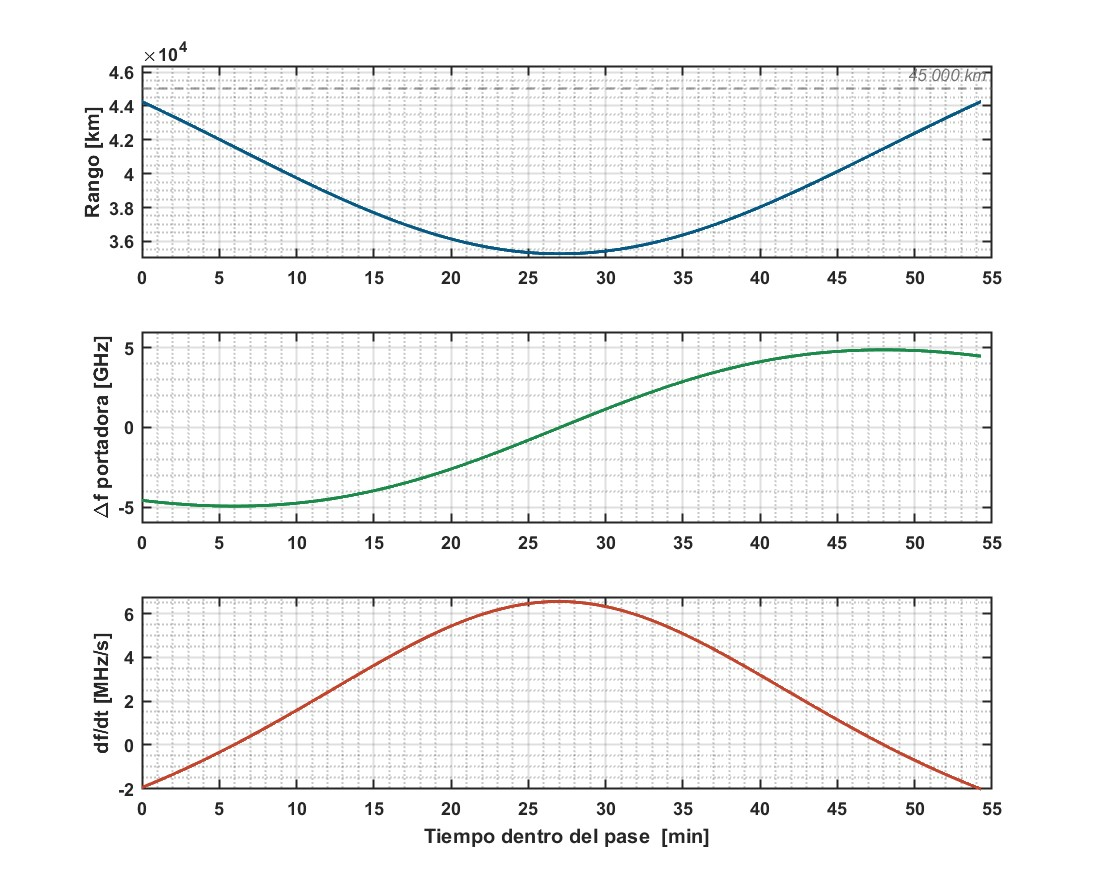
\includegraphics[width=0.94\linewidth]{DopplerGeometria}
  \caption[Doppler a lo largo de un pase LEO--GEO]{%
    Peor geometr\'ia del enlace LEO--GEO. El offset de portadora no es un valor
    fijo: barre de $-4{,}94$ a $+\SI{4.94}{\giga\hertz}$ en los
    \SI{54.3}{\minute} que dura la ventana visible, y lo hace con una
    pendiente que llega a \SI{6.55}{\mega\hertz\per\second}.}
  \label{fig:pase-doppler}
\end{figure}

El resultado, en la peor geometr\'ia, es $v_r = \SI{7.66}{\kilo\metre\per\second}$
y $a_r = \SI{10.15}{\metre\per\second\squared}$, con una ventana visible de
\SI{54.3}{\minute} por \'orbita. Esto corresponde a:

\begin{itemize}\itemsep2pt
  \item \textbf{Offset de portadora} $\abs{\Df} = \SI{4.94}{\giga\hertz}$. Es
        uno de los deterioros m\'as nocivos del canal y el que fija el requisito de captura
        del recuperador de frecuencia.
  \item \textbf{Tasa Doppler} $\abs{\fdot} = \SI{6.55}{\mega\hertz\per\second}$.
        Se analiza su contribuci\'on en el \cref{cap:tolerancias}.
  \item \textbf{Error de reloj} $\delta = \SI{25.55}{\ppm}$, equivalente a
        \SI{818}{\kilo\hertz} sobre \SI{32}{\giga\baud}. En un bloque de
        \num{3e5} s\'imbolos el muestreo se desliza \num{7.7} s\'imbolos, de
        modo que el recuperador de reloj debe ser capaz de corregir estos
        errores.
\end{itemize}

\subsection*{Requisito de captura}



De la simulaci\'on de la secci\'on anterior se obtiene un offset m\'aximo de
\SI{4.94}{\giga\hertz} en la peor geometr\'ia del pase. Cabe notar que este valor se encuentra por debajo de la
cota que se obtiene suponiendo las dos velocidades orbitales antiparalelas y
alineadas con la l\'inea de vista, $v_L + v_G =
\SI{10.66}{\kilo\metre\per\second}$ o \SI{6.88}{\giga\hertz}, que es una
situaci\'on que la geometr\'ia orbital no permite.

A este valor hay que sumarle la incerteza de los l\'aseres. El recuperador de
frecuencia compensa la diferencia entre la portadora recibida y el oscilador
local. Cada l\'aser tiene su propio error absoluto frente a la grilla en la
que se lo sintoniza, y un m\'odulo comercial sintonizable especifica
\SI{\pm1.5}{\giga\hertz} de exactitud sobre toda la banda C ~\cite{ppcl500}. Esta es una cota de peor caso sobre temperatura y
envejecimiento. Entre dos unidades puestas en el mismo canal la diferencia
t\'ipica es una fracci\'on del valor, as\'i que se adopta
\SI{1}{\giga\hertz} de residuo, y el requisito de captura resulta
\begin{equation}
  \abs{\Df}_{\mathrm{req}}
    = \underbrace{\SI{4.94}{\giga\hertz}}_{\text{Doppler, peor geometr\'ia}}
    + \underbrace{\SI{1.00}{\giga\hertz}}_{\text{residuo de l\'aseres}}
    \simeq \SI{6.0}{\giga\hertz}.
  \label{eq:requisito-captura}
\end{equation}

De esta manera, se puede asegurar que si el sistema soporta estas frecuencias, el enlace es posible.

\section{Rotaci\'on del estado de polarizaci\'on}
\label{sec:canal-sop}

Los dos telescopios no comparten una
referencia de actitud com\'un, y el \'angulo entre sus planos de polarizaci\'on
cambia a lo largo del pase. Por esta raz\'on, se tiene una rotaci\'on de los ejes de polarizaci\'on que var\'ia en el tiempo. En el formalismo de Jones, el canal es una matriz
de rotaci\'on
\begin{equation}
  \mathbf{R}(\theta) =
  \begin{bmatrix} \cos\theta & -\sin\theta \\ \sin\theta & \cos\theta \end{bmatrix},
  \qquad
  \mathbf{E}_{\mathrm{out}} = \mathbf{R}(\theta(t))\,\mathbf{E}_{\mathrm{in}},
  \label{eq:jones}
\end{equation}
que mezcla las dos tributarias sin atenuarlas.

El \'angulo se model\'o como la suma de tres contribuciones,
\begin{equation}
  \theta(t) = \theta_{0} + \dot{\theta}\,t
            + \sum_{k} A_{k}\sin(2\pi f_{k} t + \phi_{k}),
  \label{eq:sop}
\end{equation}
con significado f\'isico distinto cada una:

\begin{itemize}\itemsep2pt
  \item $\theta_0$ es el desalineamiento inicial entre las dos terminales. El
        caso m\'as exigente para el demultiplexado es $\theta_0=\pi/4$, donde
        las dos polarizaciones llegan mezcladas por igual y el ecualizador no
        tiene ninguna asimetr\'ia de la que partir.
  \item $\dot\theta$ es la deriva geom\'etrica, el macro-movimiento
        debido al cambio de orientaci\'on relativa durante el pase.
  \item El t\'ermino oscilante es el jitter del control de actitud:
        vibraciones de las ruedas de reacci\'on y de los mecanismos de
        apuntamiento.
\end{itemize}

La deriva geom\'etrica se puede acotar a trav\'es de la rotaci\'on del propio cuerpo del sat\'elite LEO. Si apunta a
nadir, da una vuelta por \'orbita para mantener la misma cara hacia la Tierra,
a la tasa orbital $\omega_L = 2\pi/T_L = \SI{1.1e-3}{\radian\per\second}$. De
esta rotaci\'on solo produce efecto la componente a lo largo de la l\'inea de vista, que
es la que hace girar el plano de polarizaci\'on, de modo que $\omega_L$ es una
cota superior. La deriva geom\'etrica queda entonces en el orden de
$\dot\theta \sim \SI{1e-3}{\radian\per\second}$ o por debajo.

En las simulaciones se utiliz\'o
$\dot\theta = \SI{5}{\radian\per\second}$, tres \'ordenes de magnitud mayor a la cota. Cabe
aclarar que esto no es una estimaci\'on f\'isica sino un valor de esfuerzo,
elegido para que la rotaci\'on sea apreciable dentro de una ventana de
simulaci\'on de microsegundos.

Las tres frecuencias referidas al jitter, \SIlist{300;1200;2000}{\hertz}, caen dentro de la banda en que se caracteriza
la micro-vibraci\'on de ruedas de reacci\'on en plataformas espaciales,
t\'ipicamente de \SIrange{10}{2000}{\hertz}~\cite{microvib2018}. Las
amplitudes tambi\'en son valores de esfuerzo mayores a los valores est\'andar.

\section{Amplificaci\'on \'optica y ruido ASE}
\label{sec:canal-ase}

La principal fuente de ruido del enlace son los amplificadores \'opticos. Ese
ruido proviene de la emisi\'on espont\'anea amplificada (ASE) del medio
activo, que en banda C es t\'ipicamente una fibra dopada con erbio (EDFA). Las
caracter\'isticas de estos amplificadores determinan la OSNR con la que llega
la se\~nal al receptor. De los dos amplificadores de la cadena domina el del receptor, porque
amplifica una se\~nal ya muy atenuada. La \cref{fig:edfa} muestra el modelo
del pre-amplificador \'optico del receptor.

\begin{figure}[H]
  \centering
  \begin{tikzpicture}[
    font=\footnotesize, >={Latex[length=2mm]},
    bl/.style ={draw, rounded corners=3pt, align=center,
                minimum height=3.2em, text width=8.6em, inner sep=3pt},
    as/.style ={draw=red!40, rounded corners=3pt, fill=red!8, align=center,
                minimum height=3.2em, text width=9.6em, inner sep=3pt},
    fl/.style ={->, thick}
  ]
    \node[bl] (a) {Amplificaci\'on\\[1pt]$E\to E\sqrt{G}$};
    \node[circle, draw, inner sep=1.2pt, right=2.2em of a] (sum) {$+$};
    \node[bl, right=2.2em of sum, text width=9.2em] (f)
          {Filtro \'optico\\[1pt]$B_o=2\Rs=\SI{64}{\giga\hertz}$};
    \node[as, below=2.0em of sum] (n)
          {Ruido ASE\\[1pt]$S_{\mathrm{pol}}=\tfrac12(F G-1)h\nu$};

    \draw[fl] ($(a.west)-(1.6em,0)$) node[left, font=\scriptsize] {$E_{rot}$} -- (a.west);
    \draw[fl] (a) -- (sum);
    \draw[fl] (sum) -- (f);
    \draw[fl] (n) -- (sum);
    \draw[fl] (f.east) -- ++(1.6em,0) node[right, font=\scriptsize] {$E_{rx}$};

    \node[below=1.1em of n, font=\scriptsize] {$G=\SI{25}{\dB}$,\quad $F=\SI{4.5}{\dB}$};
  \end{tikzpicture}
  \caption[Modelo del pre-amplificador EDFA]{%
    Pre-amplificador \'optico del receptor. El ASE se modela como un proceso
    de ruido aditivo, blanco y gaussiano, con densidad espectral de potencia
    $S_{\mathrm{pol}}$. La ganancia y la figura de ruido se justifican en el
    \cref{cap:enlace}.}
  \label{fig:edfa}
\end{figure}

La densidad espectral de potencia del ruido ASE por cada modo de
polarizaci\'on es~\cite{mello2021}
\begin{equation}
  S_{\mathrm{pol}} = \nsp\,h\nu\,(G-1) = \tfrac{1}{2}\left(F G - 1\right) h\nu ,
  \label{eq:ase}
\end{equation}
donde el factor $1/2$ proviene de la definici\'on de figura de ruido del
amplificador~\cite{agrawal2010}. Con $G=\SI{25}{\dB}$ y $F=\SI{4.5}{\dB}$
resulta $\nsp = \num{1.41}$ y
$S_{\mathrm{pol}} = \SI{5.70e-17}{\watt\per\hertz}$.

La emisi\'on espont\'anea de un EDFA no est\'a polarizada, de modo que el
medio emite por igual en los dos modos ortogonales. La
ecuaci\'on~\eqref{eq:ase} da la densidad por cada modo. Cada polarizaci\'on de
la se\~nal bate contra su propio ASE co-polarizado.

Un amplificador \'optico es seguido t\'ipicamente por un filtro que elimina la
mayor parte del ASE que cae fuera de la banda de la se\~nal. Este filtro se
model\'o como una respuesta s\'uper-gaussiana de orden~4, con un perfil plano
en la banda de inter\'es y flancos abruptos, que aproxima la respuesta de un
filtro de interferencia de pel\'icula delgada, que es la tecnolog\'ia con la
que se resuelve el filtrado \'optico en enlaces espaciales~\cite{rahmlow2018}.

El ancho de banda del filtro tiene que dejar pasar la se\~nal \'optica entera y adem\'as
absorber el desplazamiento en frecuencia. A \SI{32}{\giga\baud} con \emph{roll-off} \num{0.2} la se\~nal ocupa
\SI{19.2}{\giga\hertz} a cada lado de la portadora, y a esto se suman los
\SI{6.0}{\giga\hertz} del requisito de captura de la
\eqref{eq:requisito-captura}, lo que da unos \SI{50}{\giga\hertz} en total. Se
adopta entonces $B_o = 2\Rs = \SI{64}{\giga\hertz}$, que cubre ese presupuesto
con margen sin dejar entrar ASE de m\'as.

Por \'ultimo, la OSNR queda definida por convenci\'on como el cociente entre la
potencia total de se\~nal y el ASE total, medido en el ancho de referencia
$\Bref = \SI{12.5}{\giga\hertz}$ ~\cite{mello2021}:
\begin{equation}
  \OSNR = \frac{P_{\mathrm{sig,total}}}{2\,S_{\mathrm{pol}}\Bref}
        = \frac{P_{\mathrm{sig,pol}}}{S_{\mathrm{pol}}\Bref}.
  \label{eq:osnr-def}
\end{equation}


\section{Conclusiones}
\label{sec:canal-conclusiones}

En este cap\'itulo se present\'o el modelo del canal LEO--GEO usado en este
trabajo. La \cref{tab:canal-parametros} re\'une los par\'ametros con los que
se lo simul\'o.

\begin{table}[!htb]
\centering

\begin{tabular}{llc}
\toprule
\textbf{Bloque} & \textbf{Par\'ametro} & \textbf{Valor} \\
\midrule
Geometr\'ia        & Distancia de dise\~no            & \SI{45000}{\kilo\metre} \\
                   & P\'erdida neta del enlace        & \SI{73.40}{\dB}         \\
\addlinespace
Doppler            & Offset de portadora m\'aximo     & \SI{4.94}{\giga\hertz}  \\
                   & Requisito de captura             & \SI{6.0}{\giga\hertz}   \\
                   & Tasa Doppler m\'axima            & \SI{6.55}{\mega\hertz\per\second} \\
                   & Error de reloj m\'aximo (SFO)    & \SI{25.55}{\ppm}        \\
\addlinespace
Polarizaci\'on     & Deriva geom\'etrica (cota)         & \SI{1e-3}{\radian\per\second} \\
                   & Deriva usada en la simulaci\'on  & \SI{5}{\radian\per\second}    \\
                   & Jitter de actitud                & \SIlist{300;1200;2000}{\hertz} \\
\addlinespace
Ruido \'optico     & Ganancia del pre-amplificador    & \SI{25}{\dB}            \\
                   & Figura de ruido                  & \SI{4.5}{\dB}           \\
                   & Ancho del filtro \'optico        & \SI{64}{\giga\hertz}    \\
\bottomrule
\end{tabular}
\caption[Par\'ametros del modelo de canal]{%
Par\'ametros del modelo de canal LEO--GEO. Los valores de Doppler corresponden
a la geometr\'ia m\'as desfavorable del pase.}

\label{tab:canal-parametros}
\end{table}

Con estos valores de referencia, se analizan en los cap\'itulos siguientes las tolerancias y m\'argenes que se tienen presentes
en el sistema, y qu\'e efectos son m\'as significativos que otros.

